\documentclass{boi2014-fi}

\usepackage{enumitem}
\usepackage{wrapfig}
\usepackage{mathtools}
\usepackage{tikz}

\renewcommand{\DayNum}{1}
\renewcommand{\TaskCode}{coprobber}
\renewcommand{\TaskName}{Rosvo ja poliisi}
\renewcommand{\TaskVersion}{1.3}

\renewcommand{\labelitemii}{$\circ$}
\newcommand{\constant}[1]{{\tt #1}}

\begin{document}
    \begin{wrapfigure}[8]{r}{6cm}
        \vspace{-24pt}
		\includegraphics[width=6cm]{\TaskCode.jpeg}
	\end{wrapfigure}
    
    Bytemoren kaupungissa rikosten määrä on saavuttamassa kaikkien aikojen
    huipun. Muun rötöstelyn lisäksi ryöstöjä tapahtuu joka päivä.
    Joka kerta kun ryöstö tapahtuu, on yksittäisen partioivan poliisin
    tehtävä jahdata rosvo kiinni kadunkulmia yhdistäviä kapeita kujia
    pitkin. Ikävä kyllä, useimmiten rosvot pääsevät pakoon takaa-ajajiltaan,
    koska he tuntevat kaupungin paljon poliisia paremmin.

    Bytemoren kaupungin poliisilaitos järjestää kokouksen, jonka tehtävänä
    on vähentää rikollisuutta. Yksi aloitteista on käyttää tietokonetta
    apuna rosvojen jahtaamisessa. Tätä varten poliisilaitos on tehnyt tarkan
    kartan kaupungista. Nyt he tarvitsevat tietokoneohjelmaa
    jahtausstrategioiden päättämiseen.
    
    Rosvojahti jossa yksi poliisi jahtaa yhtä rosvoa mallinnetaan seuraavasti:
    \begin{enumerate}
        \item Poliisi valitsee kadunkulman jossa partioi.
        \item Rosvo valitsee kadunkulman jossa ryöstö tehdään (hän tietää
            aina missä poliisi on). Tästä lähtien oletetaan aina että sekä
            poliisi että rosvo tietävät missä kumpikin ovat.
        \item Poliisi siirtyy siirrollaan joko viereiseen kadunkulmaan
            (sellaiseen johon kulkee nykyisestä kuja) tai odottaa paikallaan (ei siirry).
        \item Rosvo siirtyy aina vuorollaan viereiseen kadunkulmaan. Huomaa,
            että toisin kuin poliisit, rosvot eivät voi odottaa paikallaan.
            Heidän vaistonsa saa heidät jatkamaan juoksua.
        \item Poliisi ja rosvo tekevät siirtoja vuorotellen (aloittaen poliisista)
            kunnes yksi seuraavista tapahtuu:
        \begin{enumerate}
            \item sama tilanne toistuu (tilanne määritellään rosvon ja poliisin
                sijainteina ja sillä, kenen vuoro on seuraavaksi). Tämä vastaa
                sitä, että rosvo voi vältellä poliisia loputtomasti, joten
                rosvo pääsee pakoon;
            \item poliisi ja rosvo ovat samassa kadunkulmassa kumman tahansa
                vuoron jälkeen. Tässä tapauksessa poliisi saa rosvon kiinni.
        \end{enumerate}
    \end{enumerate}

    \Task
    Sinun tulee kirjoittaa ohjelma, jolle annetaan kaupungin kartta, ja joka
    päättelee onko poliisin mahdollista saada rosvo kiinni, ja jos on, osaa
    kertoa millä poliisin siirroilla rosvo saadaan kiinni.
    
    Ohjelmasi on oletettava että rosvo liikkuu optimaalisesti.

    \Implementation
    Sinun tulee toteuttaa kaksi funktiota:
    \begin{itemize}
        \item \method{start(N, A)} joka ottaa seuraavat parametrit:
            \begin{itemize}
                \item $N$ --- kadunkulmien lukumäärä (kadunkulmat numeroidaan
                    luvuilla $0 \ldots N-1$);
                \item $A$ --- kaksiulotteinen taulukko joka määrittelee kujat:
                Kaikille $0 \le i, j \le N-1$,
                    $$
                        A[i, j] \text{ on }
                        \begin{dcases*}
                            \texttt{false}, & jos kadunkulmia $i$ ja $j$ ei yhdistä kuja
                                \\
                            \texttt{true}, & jos kadunkulmia $i$ ja $j$ yhdistää kuja
                        \end{dcases*}
                    $$
                    Kaikki kujat ovat kaksisuuntaisia (siis $A[i, j] = A[j, i]$
                    kaikille kadunkulmille $i$ ja $j$) ja mikään kuja ei liitä
                    kadunkulmaa itseensä (siis $A[i, i]$ on \texttt{false} kaikille
                    kadunkulmille $i$). Voit myös olettaa että voit saavuttaa minkä
                    tahansa kadunkulman mistä tahansa toisesta kadunkulmasta liikkumalla
                    kujia pitkin.
            \end{itemize}

        Mikäli poliisin on mahdollista saada rosvo kiinni annetussa kartassa,
        funktion \method{start} tulisi palauttaa sen kadunkulman tunnusnumero
        jossa poliisi päättää partioida. Muussa tapauksessa sen tulisi palauttaa $-1$.
        
        \item \method{nextMove(R)} joka ottaa parametrina rosvon nykyisen kadunkulman
            tunnusnumeron $R$ ja palauttaa sen kadunkulman tunnusnumeron missä
            poliisi on siirtonsa jälkeen.
    \end{itemize}

    Funktiota \method{start} kutsutaan täsmälleen kerran ennen kuin kutsuja
    funktioon \method{nextMove} tehdään. Mikäli \method{start} palauttaa $-1$,
    niin funktiota \method{nextMove} ei kutsuta. Muussa tapauksessa funktiota
    \method{nextMove} kutsutaan toistuvasti kunnes jahti on ohi. Tarkemmin
    ohjelma loppuu kun yksi seuraavista tapahtuu:
    \begin{itemize}
        \item \method{nextMove} palauttaa virheellisen siirron;
        \item tilanne toistuu;
        \item poliisi saa rosvon kiinni.
    \end{itemize}
    
    \Example
    \begin{wrapfigure}[4]{r}{2cm}
        \vspace{-0.5cm}
        \centering
        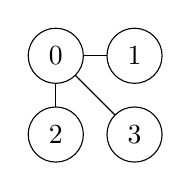
\begin{tikzpicture}
        \draw (0,1) -- (0,0);
        \draw (0,1) -- (1,0);
        \draw (0,1) -- (1,1);
        \foreach \x in {0,1} \foreach \y in {0,1}
            \draw (\x,\y) node[circle,draw,fill=white,inner sep=0,minimum size=0.7cm] {\pgfmathparse{int(2-2*\y+\x)}\pgfmathresult};
        \end{tikzpicture}
    \end{wrapfigure}
    Tarkastellaan oikealla olevaa esimerkkiä.
    Tässä tapauksessa mikä tahansa kadunkulma on hyvä aloituskohta poliisille.
    Jos hän aloittaa kadunkulmasta 0, hän voi odottaa ensimmäisen siirtonsa ajan
    ja rosvo juoksee hänen luokseen.
    Jos taas hän aloittaa mistä tahansa muusta kadunkulmasta,
    hän voi odottaa, kunnes rosvo siirtyy kadunkulmaan 0, ja siirtyä sitten sinne.

    Tässä on esimerkki tapahtumien kulusta:

    \begin{tabular}{|l|c|}
        \hline
            {\bf Funktiokutsu} & {\bf Palauttaa} \\
        \hline
            \method{start(4, [[0, 1, 1, 1], [1, 0, 0, 0], [1, 0, 0, 0], [1, 0, 0, 0]])} &
            \constant{3} \\
        \hline
            \method{nextMove(1)} & \constant{3} \\
        \hline
            \method{nextMove(0)} & \constant{0} \\
        \hline
    \end{tabular}

    Huomaa, että funktion \method{start} kutsussa ylhäällä
    \constant{0} tarkoittaa samaa kuin \constant{false} ja
    \constant{1} tarkoittaa samaa kuin \constant{true} lyhyyden vuoksi.

    \Scoring
    \begin{description}
        \item[Osatehtävä 1 (16 pistettä):] $2 \le N \le 500$.
        Jokaisen kahden kadunkulman välillä on tasan yksi polku.        
        \item[Osatehtävä 2 (14 pistettä):] $2 \le N \le 500$. Kadunkulmien ja
        kujien verkosto muodostaa ruudukkorakenteen. Ruudukossa on vähintään
        kaksi riviä ja saraketta, ja kadunkulmien numerointi noudattaa
        alla olevaa sääntöä.
        \begin{figure}[h!]
           \centering
           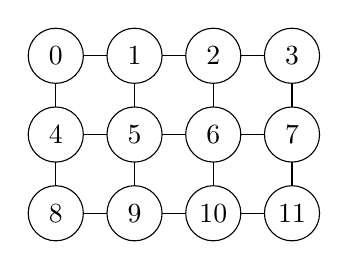
\begin{tikzpicture}
            \draw (0,0) grid (3,2);
            \foreach \x in {0,1,2,3} \foreach \y in {0,1,2}
                \draw (\x,\y) node[circle,draw,fill=white,inner sep=0,minimum size=0.7cm] {\pgfmathparse{int(8-4*\y+\x)}\pgfmathresult};
           \end{tikzpicture}
        \end{figure}
        \item[Osatehtävä 3 (30 pistettä):] $2 \le N \le 100$.
        \item[Osatehtävä 4 (40 pistettä):] $2 \le N \le 500$.
    \end{description}

    Ratkaisusi tulisi täyttää seuraavat kaksi vaatimusta:
    \begin{enumerate}
        \item määrittää oikein voiko poliisi saada rosvon kiinni;
        \item onnistuu ottamaan rosvon kiinni tekemällä poliisin siirrot
    \end{enumerate}
    
    Osatehtävissä 1 ja 2 ratkaisusi täytyy toteuttaa molemmat vaatimukset
    saadakseen pisteitä.
    Osatehtävissä 3 ja 4 ratkaisut jotka toteuttavat vain ensimmäisen vaatimuksen
    saavat 30\% osatehtävän pisteistä. 
    Mikäli ratkaisusi tähtää vain osittaisiin pisteisiin, voit lopettaa
    ohjelman tulostamalla virheellisen siirron (esimerkiksi palauttaa $-1$
    funktiossa \method{nextMove}).
    
    Huomaa että perusvaatimukset (aika- ja muistirajat, ei ajonaikaisia virheitä)
    täytyy toteutua jotta saisit yhtään pisteitä.
    
    \Constraints
    
    \begin{description}
        \item[Aikaraja:] 1.5 s.
        \item[Muistiraja:] 256 MB.
    \end{description}

    \Experimentation
    Koneellasi oleva esimerkkitarkastaja lukee tietoa standardisyötteestä.
    Syötteen ensimmäisellä rivillä tulee olla kokonaisluku $N$ ---
    kadunkulmien lukumäärä. Seuraavilla $N$ rivillä tulee olla
    vierusmatriisi $A$. Jokaisella tällaisella rivillä tulee olla $N$ lukua,
    joista jokainen on 0 tai 1.
    Matriisin tulee olla symmetrinen ja päädiagonaalin kaikkien arvojen
    tulee olla nollia.

    Seuraavalla rivillä tulee olla luku 1, jos poliisi pystyy saamaan kiinni ryöstäjän,
    ja muuten luku 0.

    Jos poliisi pystyy ottamaan rosvon kiinni, täytyy tulla vielä $N$ riviä,
    jotka kuvaavat rosvon strategian.
    Jokaisella tällaisella rivillä tulee olla $N+1$ kokonaislukua 0:n ja $N-1$:n välillä.
    Rivin $r$ sarakkeen $c$ arvo, jossa $c < N$, vastaa tilannetta,
    jossa on rosvon vuoro, poliisi on kadunkulmassa $r$ ja rosvo on
    kadunkulmassa $c$. Arvo kuvaa kadunkulman, johon rosvon on siirryttävä.
    Päädiagonaalin arvoista ei välitetä, koska ne vastaavat tilanteita,
    joissa rosvo ja poliisi ovat samassa kadunkulmassa.
    Rivin $r$ viimeinen arvo määrittelee rosvon aloituskadunkulman jos poliisin
    aloituskadunkulma on $r$.

    Tässä on esimerkkisyöte tarkastajalle, joka kuvaa kolme kadunkulmaa,
    jotka on yhdistetty toisiinsa:

    \begin{center}
        \begin{tabular}{p{4cm}}
            {\tt
                3 \newline
                0 1 1 \newline
                1 0 1 \newline
                1 1 0 \newline
                1 \newline
                0 2 1 2 \newline
                2 0 0 2 \newline
                1 0 0 1 \newline
            }
        \end{tabular}
    \end{center}

    Ja tässä on syöte, joka täsmää yllä olevan tehtävänannon esimerkkiin:

    \begin{center}
        \begin{tabular}{p{4cm}}
            {\tt
                4 \newline
                0 1 1 1 \newline
                1 0 0 0 \newline
                1 0 0 0 \newline
                1 0 0 0 \newline
                1 \newline
                0 0 0 0 1 \newline
                2 0 0 0 2 \newline
                3 0 0 0 3 \newline
                1 0 0 0 1 \newline
            }
        \end{tabular}
    \end{center}
\end{document}
